\section{Partial Design Logs}
Some significant design logs were kept. Here is a sample of those:

Started EZ USB dev board design
Decided on 50x50mm 6-layer PCB + stencils, whichi will cost ~\$19 + ship from jlcpcb
There is no footprint or symbol for the EZ USB in kicad -> Imported from samacsys and verified footprint \& symbol briefly

For the crystal Oscilator, a 19.2Mhz crystal \& appropriate load caps are required. Added to mouser cart.
https://www.mouser.com/ProductDetail/ECS/ECS-192-7-36B-CKY-TR?qs=l7cgNqFNU1gBRjqdHCSS7A%3D%3D
CC0402BRNPO9BN7R0

For the watchdog timer, a 32khz crystal is required. These crystals are expensive (>\$1), So I'm omitting them.

The clock source selection requires a pull up or pull down on FSLC pins. Placing a solder bridge jumper to gnd, and a resistor network for pull up.
Pulling up to "CVDDQ" because that is the IO's power domain.

Now considering the connector between the pcb and the computer. For USB 2.0, this would be the Micro USB or Mini USB, or other connectors.
https://community.infineon.com/t5/Knowledge-Base-Articles/Designing-Type-C-products-based-on-EZ-USB-FX3-and-CX3/ta-p/251806


USB C is somewhat complex to implement (requiring an additional MUX chip) but can provide more power.
Do we need more power? -> The EZ USB draws 200mA for the core, 60mA for the USB, and up to 16mA per IO, (but this much likely isn't necessary).
We are planning to do 32 data + clk + some control lines of I/O, so if we call that 36 lines @ 16mA then the total (max) power draw is 640mA for the I/O.
This gives a total (absolute max) power draw for the chip at 836mA*

It is worth noting, that the chip operates at a core voltage of 1.2v, and I/O voltages of 3.3v(by our selection).

836mA is below the USB 3.0 type A spec of 900mA, so we could safely use linear voltage regulators for these power supplies, and still have sufficient power delivery from a usb 3.0 type A port.

Assuming 80\% efficiency of the buck regulators I intend to use, we will need (1.2v/5v)/.8 * 260mA + (3.3v/5v)/.8 * 640mA = 78ma + 528ma = 606mA (maximum) of power from the usb port. This leaves a decent margin on the power a USB 3 port can provide.

So, all of that said, I believe that the best choice for a usb plug for our device is going to be a USB 3 A/B plug, and then we purchase USB 3 type A and C to USB 3 AB cables to allow the device to be used on either a desktop with 3.0 type A ports, or a laptop with type c ports.

By using the type AB plug, we avoid the added complexity and cost of type C and the connection switching MUX.

Ordered the appropriate receptacles from aliexpress. (The receptacles were \$3/ea on mouser, compared to 40 for \$5 shipped on aliexpress.)
Ordered appropriate cables from amazon


\section{Features of the custom development board design}
\begin{itemize}
	\item What you see today is the proof-of-concept/development board we designed.
	\item The chip at the heart of the board is the STM32G474, with relevant features:
	\begin{itemize}
		\item 5 x ADC, 5MSPS @ 12bit, up to 25MSPS with chaining. This allows effective measurement of analog signals up to $\sim$5MHz at full resolution.
		\item 42 ADC Channels
		\item 7 x 12 bit DAC Channels, 15MSPS
		\item Cortex M4 CPU with a vector processing unit @ 170MHz
		\item 128K SRAM, 512KB Program Memory
		\item External high speed SRAM up to 512MB (not fitted) - This allows for storage of huge sample depths - 340Mpts at full resolution.
	\end{itemize}
	\item The board adds these external components:
	\begin{itemize}
		\item On board SD card slot for saving waveform data
		\item LCD Display, 4 buttons, and a rotary encoder for control
		\item OPAMP output buffers for output, allowing for the signal generator functionality to drive 50 ohm loads at an expanded range of 5 volts. This does not include negative voltages, as they are not often used in the low-voltage design space that our product targets.
		\item OPAMP input buffers for the analog channels, allowing input impedances of up to 20M Ohms without unduly loading down the circuit under test over the whole frequency range. This allows the use of standard 10:1 oscilloscope probes
		\item STM32G030 MCU for dedicated control of the LCD and touchscreen features; used for offloading processing from the main CPU
		\item Switching Voltage Regulator for battery power, expected 90\% efficient, battery input voltages of up to 14V allowed.
	\end{itemize}
\end{itemize}

The EZ USB Board was completed, with over 900 solder joints and 8 layers.

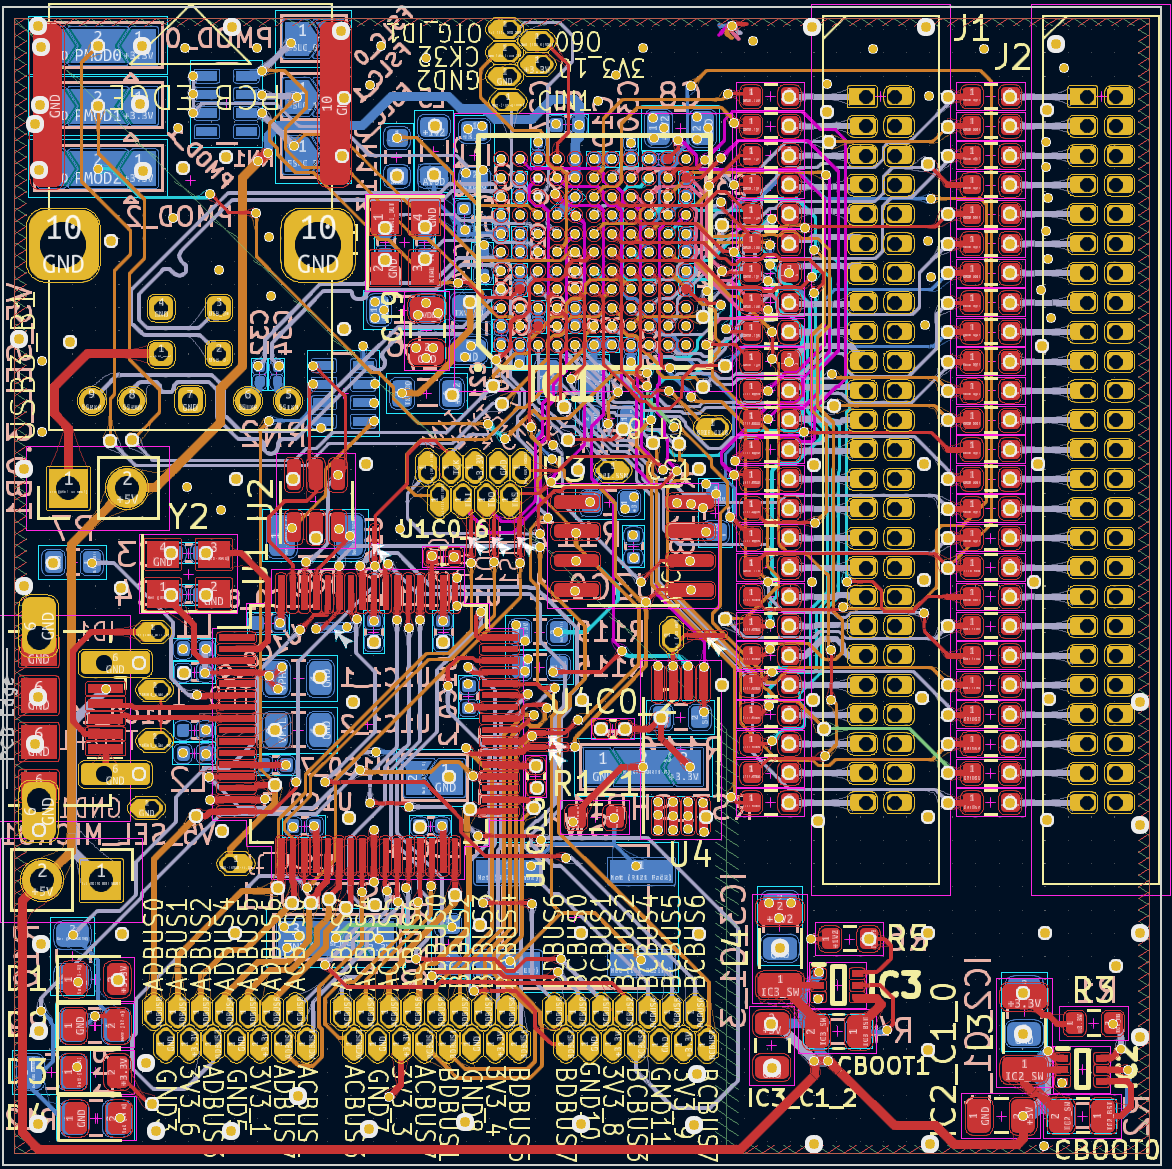
\includegraphics{ezusb}

\section{BOM for complete project}
\begin{itemize}
	\item \$0.81 PCB
	\item \$4.36 STM32G474VEH6
	\item \$0.47 Rotary encoder with knob
	\item \$0.72 10mhz/1pA bias current fast quad opamps
	\item \$0.32 STM32G030
	\item \$2.80 2.8" 240x320 TFT Touch Display
	\item \$0.09 Microsd card slot
	\item \$0.32 Trim Potentiometers
	\item \$0.27 Voltage Regulator
	\item \$0.30 Buttons
	\item \$0.06 Volume Wheel
	\item \~\$1 discreet components (resistors, capacitors, mosfets, diodes, LEDs, inductors, precision crystal resonator)
	\item \$3.00 256Mb flash memory chips x 2 (Optional, not fitted)
	\item \$8.46 256Mb external PSRAM x2 (Optional, not fitted)
	\item \$4.84 1.27mm programming cable header (Development only, not be be fitted in production)
\end{itemize}

Total parts cost of ~\$11.57 per unit, at 1K units, omitting optional components.

Assembly cost: \$0.95/ea + \$50 setup fee + \$15 Stencil fee

Total cost for each complete unit: \$12.60
(Plus shipping, tariffs, etc)

This, of course, does not include a case or battery. The battery could be a few dollars, and a proper plastic injection molded case would have a unit cost of about \$1 all inclusive, that includes labor to install the electronics and test the device.... After ~\$6000 for creation of the molds. (Jeremy's family used to own a plastic molding company, where he did some CAD and Mold building work. This price is an estimate from that experience.)

All together, in quantity, after shipping costs, we could call it \$15/ea assembled. There are some upfront costs that would make the early units more expensive. This would suggest a minimum retail price of ~\$45 for a viable company.

This is about half the cost of other, dramatically less capable products on the market. IE, DSO Nano, FNRSI, Hantek offerings with only one or two channels at 5msps or less, no (or poor) measurement software to integrate with, no signal generator, and lower impedance probes, IE 100Kohm-1Meg, that make them unsuited to measure sensitive signals.

\section{Project Result}
Although we did not accomplish everything we set out to do, we did successfully create a working product to demo that "Proofs" all the concepts in the design.

The main part of the project that is missing is the EZ USB board to aggregate data from multiple sources. This was not strictly within our control to prevent, as Infineon shut down the software servers without alternatives or notice, not us. Certainly, the software will become available again sometimes soon, as Infineon still offers the Cypress catalog, including the EZ USB chip in our project. With a little time, we are sure that Infineon could be contacted and would provide the needed files also. Once these are available, our software work was already nearly complete.

The final analog tile provides all of the 5 fast ADC devices on multiple channels, and the 4 fast DAC channels for signal generation. This functionality is fully implemented in the design.

The software integration with NGSCope client went very smoothly, and provides a huge suite of tools to perform analysis on the loaded data.

The analog tile board successfully implements power supplies, input and output buffers at 10Meg Ohm input/50 ohm output impedances, output signal on/off switching with FET Switches, and use of an LCD for setting options.

Overall, we believe that we did significantly more work on this project than most other teams in capstone, and applied a wealth of real-world design tools in this project. We faced some unique challenges between the software shutdown issues and team member illness, so the project lacks the completeness and polish that we would otherwise like. We beleive this project presents a solid point to push into a feature complete design that would be an excellent contender in the market.